\documentclass{article}
\usepackage[utf8]{inputenc}
\usepackage{amsmath, amssymb, amsthm}
\usepackage{algorithm,algpseudocode}
\usepackage{float}
\usepackage[shortlabels]{enumitem}
\usepackage{graphicx} % Required for inserting images
\title{MATH512 - Project 4}
\author{Wasif Ahmed, Haoxiang Deng, Jacob Fein-Ashley, Kanav Malhotra, Longzhe Yang}
\date{April 2024}

\begin{document}

\maketitle

\section*{Question 1}

Refer to figure~\ref{fig:abssum} and ~\ref{fig:sqrsum}. 

\begin{figure}[H]
    \centering
    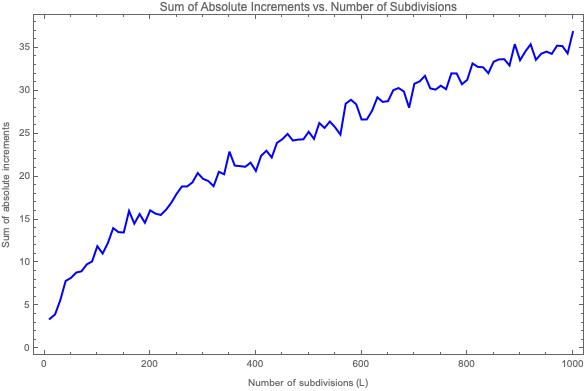
\includegraphics[scale=0.6]{imgs/AbsSum.jpeg}
    \caption{$|\delta W_i|$}
    \label{fig:abssum}
\end{figure}

\begin{figure}[H]
    \centering
    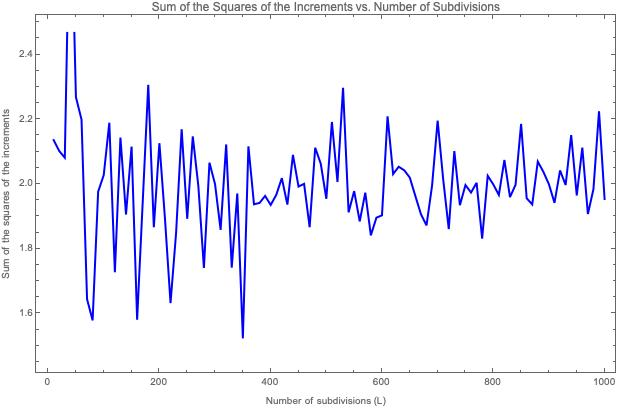
\includegraphics[scale=0.6]{imgs/SqrSum.jpeg}
    \caption{$\delta W_i^2$}
    \label{fig:sqrsum}
\end{figure}
Notice that as the $L$ parameter increases, the $|\delta W_i|$ term is unbounded while $\delta W_i^2$ converges to $2$ in probability.

\section*{Question 2}

\begin{enumerate}
    \item 
        \begin{figure}[H]
            \centering
            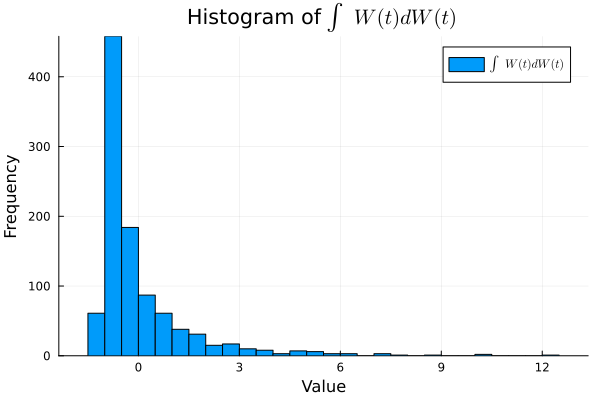
\includegraphics[scale=0.6]{imgs/2a.png}
            \caption{2a}
            \label{fig:2a}
        \end{figure}

    \item 
        \begin{figure}[H]
            \centering
            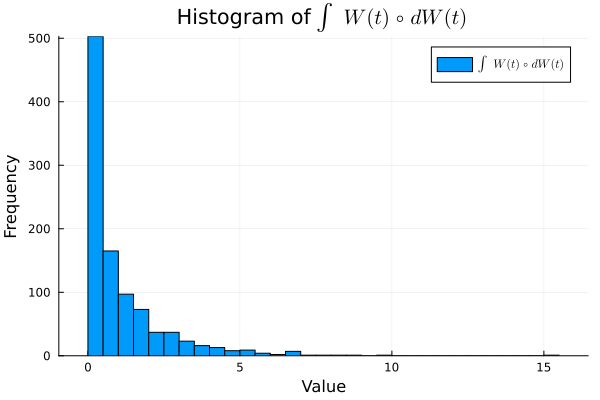
\includegraphics[scale=0.6]{imgs/2b.png}
            \caption{2b}
            \label{fig:2b}
        \end{figure}
    \item
        \begin{figure}[H]
            \centering
            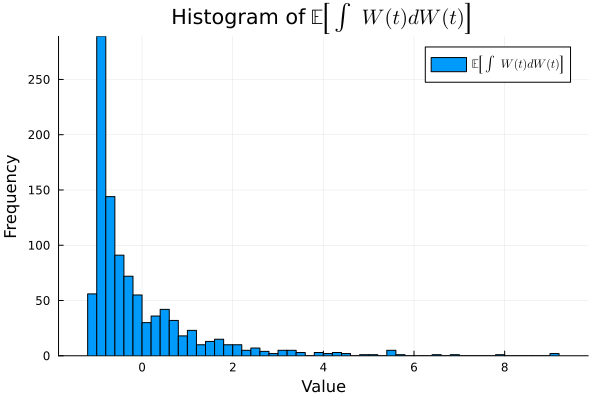
\includegraphics[scale=0.6]{imgs/2c.png}
            \caption{2c}
            \label{fig:2c}
        \end{figure}
    \item
        \begin{figure}[H]
            \centering
            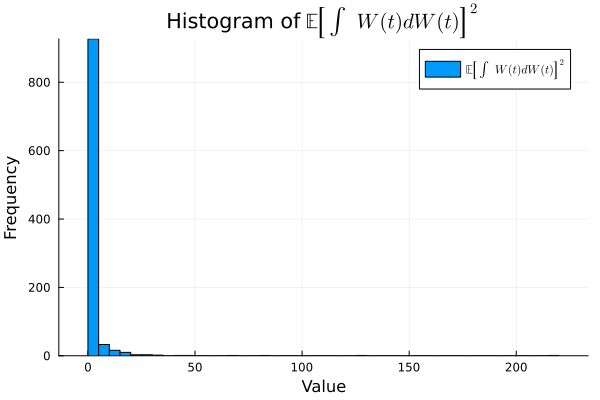
\includegraphics[scale=0.6]{imgs/2d.png}
            \caption{2d}
            \label{fig:2d}
        \end{figure}
    \item
        \begin{figure}[H]
            \centering
            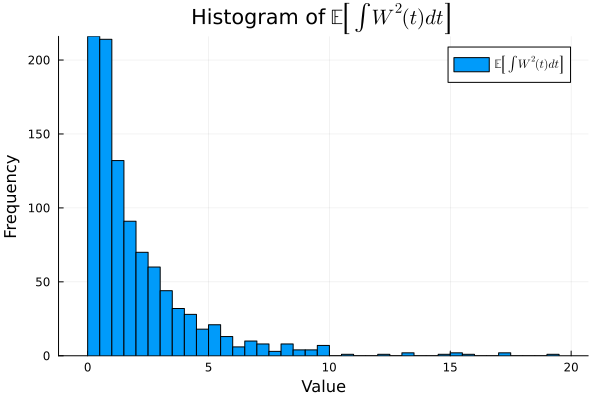
\includegraphics[scale=0.6]{imgs/2e.png}
            \caption{2e}
            \label{fig:2e}
        \end{figure}

    \item 
        \begin{figure}[H]
            \centering
            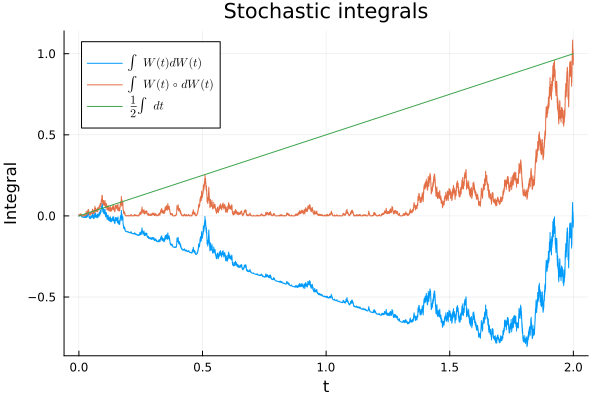
\includegraphics[scale=0.6]{imgs/2f.png}
            \caption{2f}
            \label{fig:2f}
        \end{figure}
\end{enumerate}

\section*{Question 3}
 \textbf{Objective:} Analyze the weak and strong order of convergence of the EM method for solving the given SDE:
    \[
    dX(t) = \mu X(t) dt + \sigma X(t) dW(t), \quad X(0)=3, \quad \mu=2 , \quad \sigma=0.10
    \]

    \begin{itemize}
        \item \textbf{Weak order of convergence equal to 1:} to show that 
         \[
    |E[X_1]-E[X(1)]|=C\Delta t 
    \]
        \item \textbf{Strong order of convergence equal to 0.5:} to show that
         \[
    E|X_1-X(1)|=C\Delta t^{0.5} 
    \]
    \end{itemize}
    where ${X_1}$ stands for the exact solution and X(1) stands for the estimated solution.
    
\textbf{Weak Order of Convergence} focuses on the \textbf{expected values} of the numerical solution compared to the exact solution
    \[
    |E[X_1]-E[X(1)]|=C\Delta t 
    \]
    
    \begin{itemize}
        \item A plot of the error versus \(\Delta t\) for the  weak order of convergence of 1. 
        \begin{figure}[H]
            \centering
            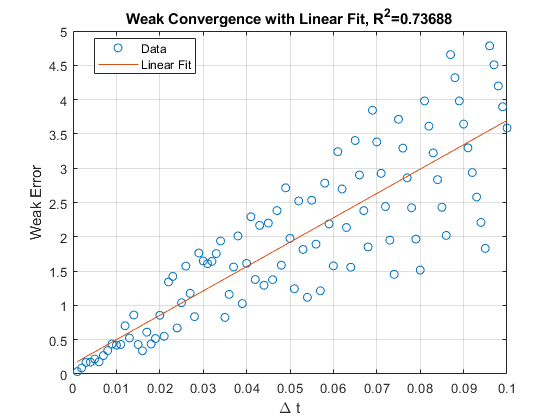
\includegraphics[scale=0.4]{imgs/fig1.png}
            \label{fig:3a}
       \end{figure}
        
    \end{itemize}
    
\textbf{Strong Order of Convergence to 0.5}  is concerned with the \textbf{pathwise accuracy}, evaluating how closely the numerical solution follows individual realizations of the exact solution.
    \[
    E|X_1-X(1)|=C\Delta t^{0.5} 
    \]
    \begin{itemize}
        \item A plot of the error versus \(\Delta t^{0.5}\) for the  strong order of convergence of 0.5. 
            
             \begin{figure}[H]
            \centering
            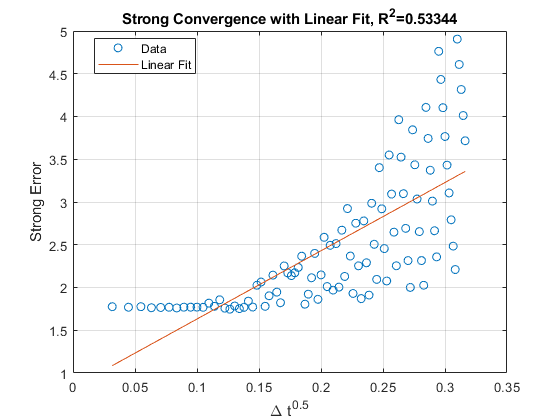
\includegraphics[scale=0.4]{imgs/fig2.png}
            \label{fig:3a}
             \end{figure}
                
            
    \end{itemize}


\section*{Question 4}
\begin{figure}[H]
    \centering
    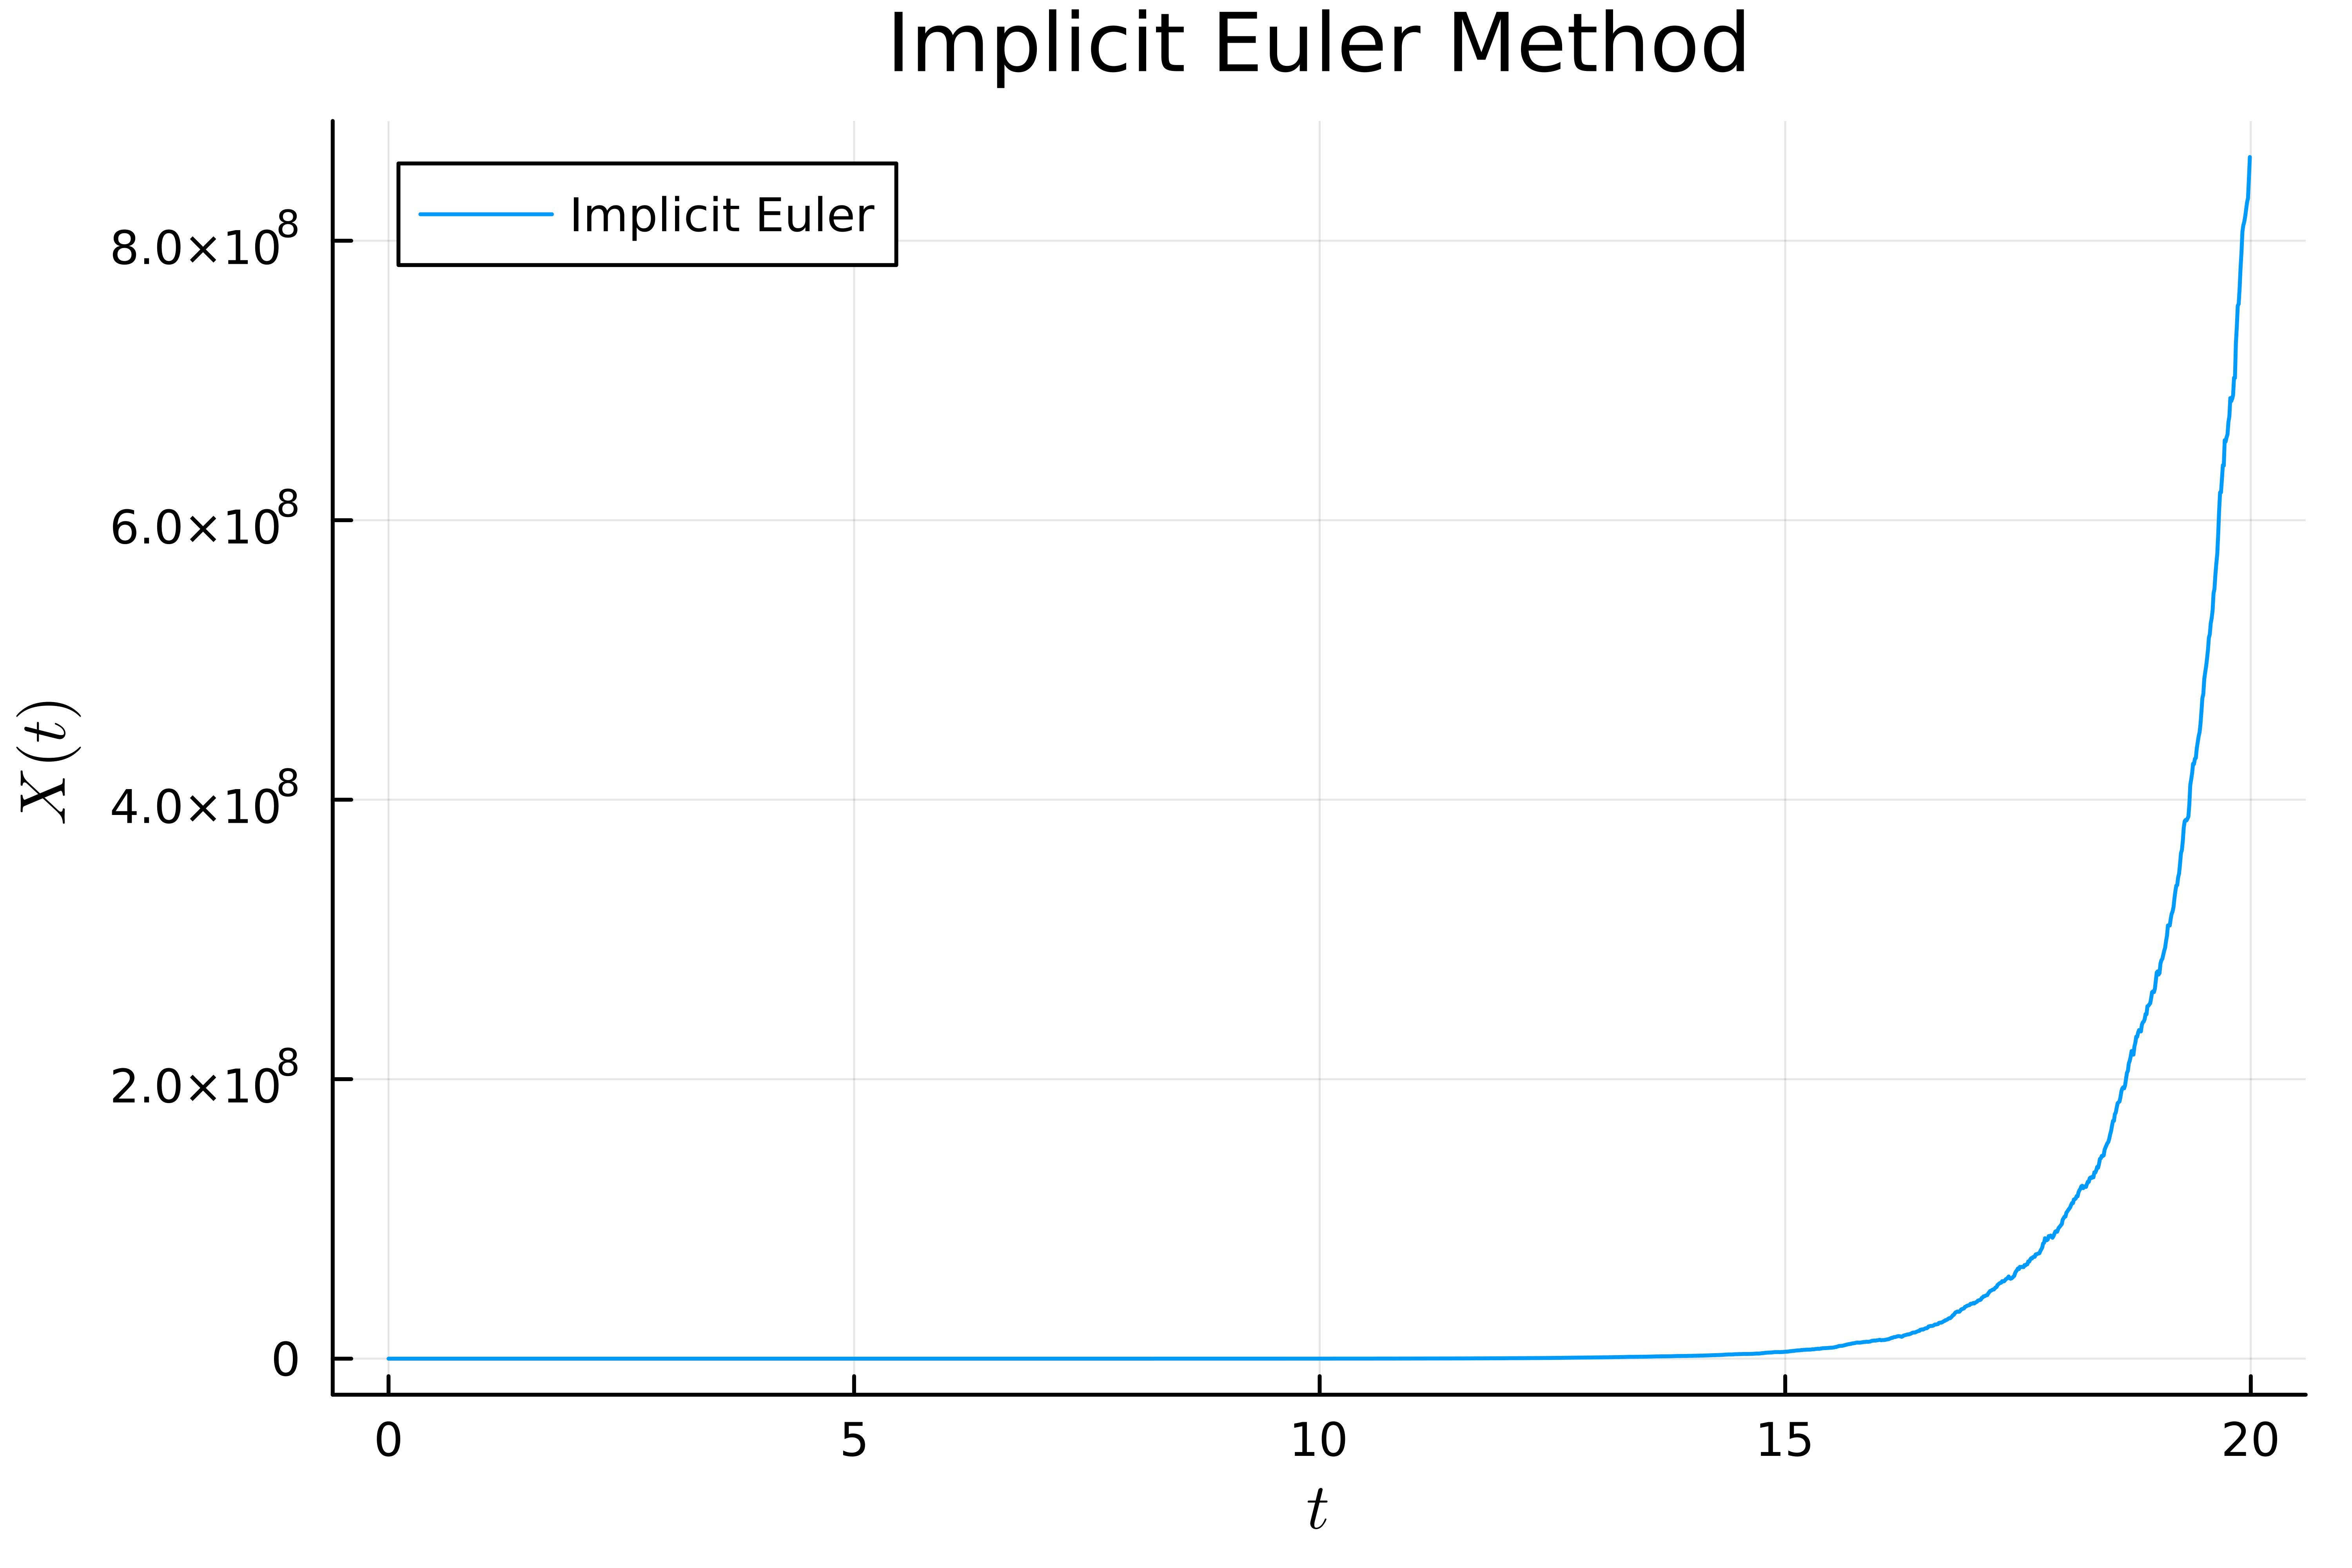
\includegraphics[scale=0.05]{imgs/4implicit_euler.png}
    \caption{Implicit Euler}
    \label{fig:impliciteuler}
\end{figure}

\begin{figure}[H]
    \centering
    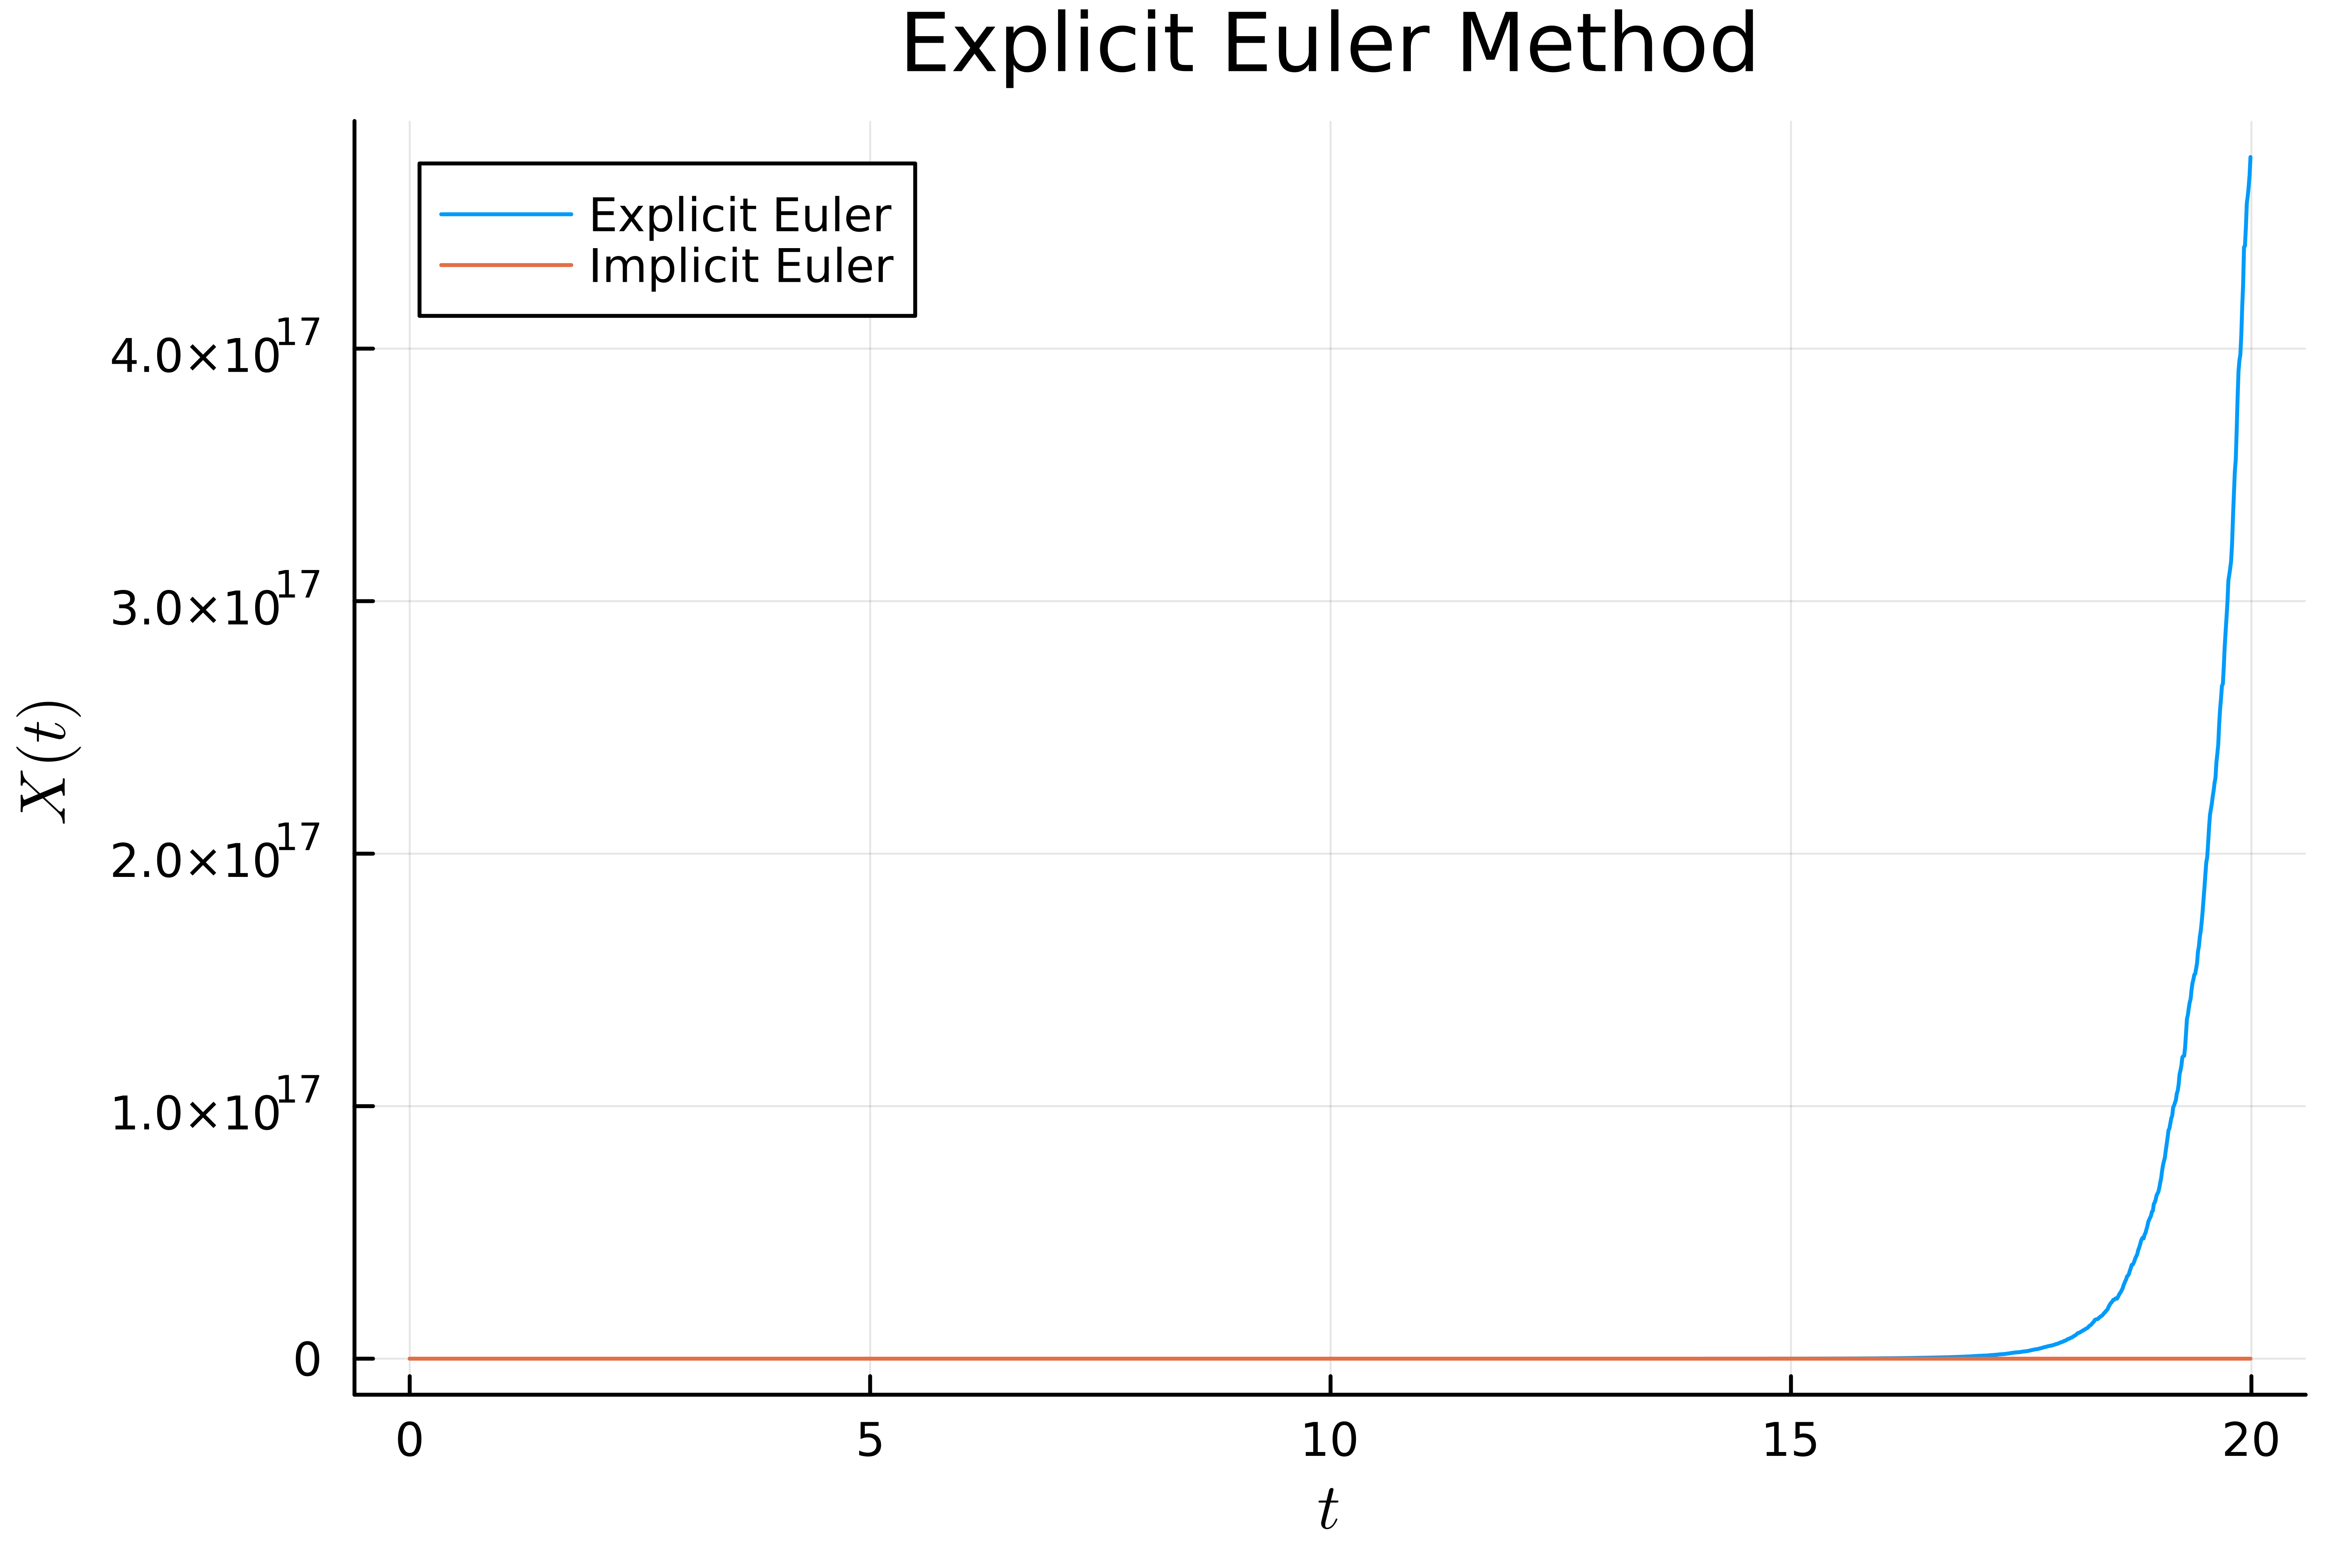
\includegraphics[scale=0.05]{imgs/4explicit_euler.png}
    \caption{Explicit Euler}
    \label{fig:expliciteuler}
\end{figure}

\begin{figure}[H]
    \centering
    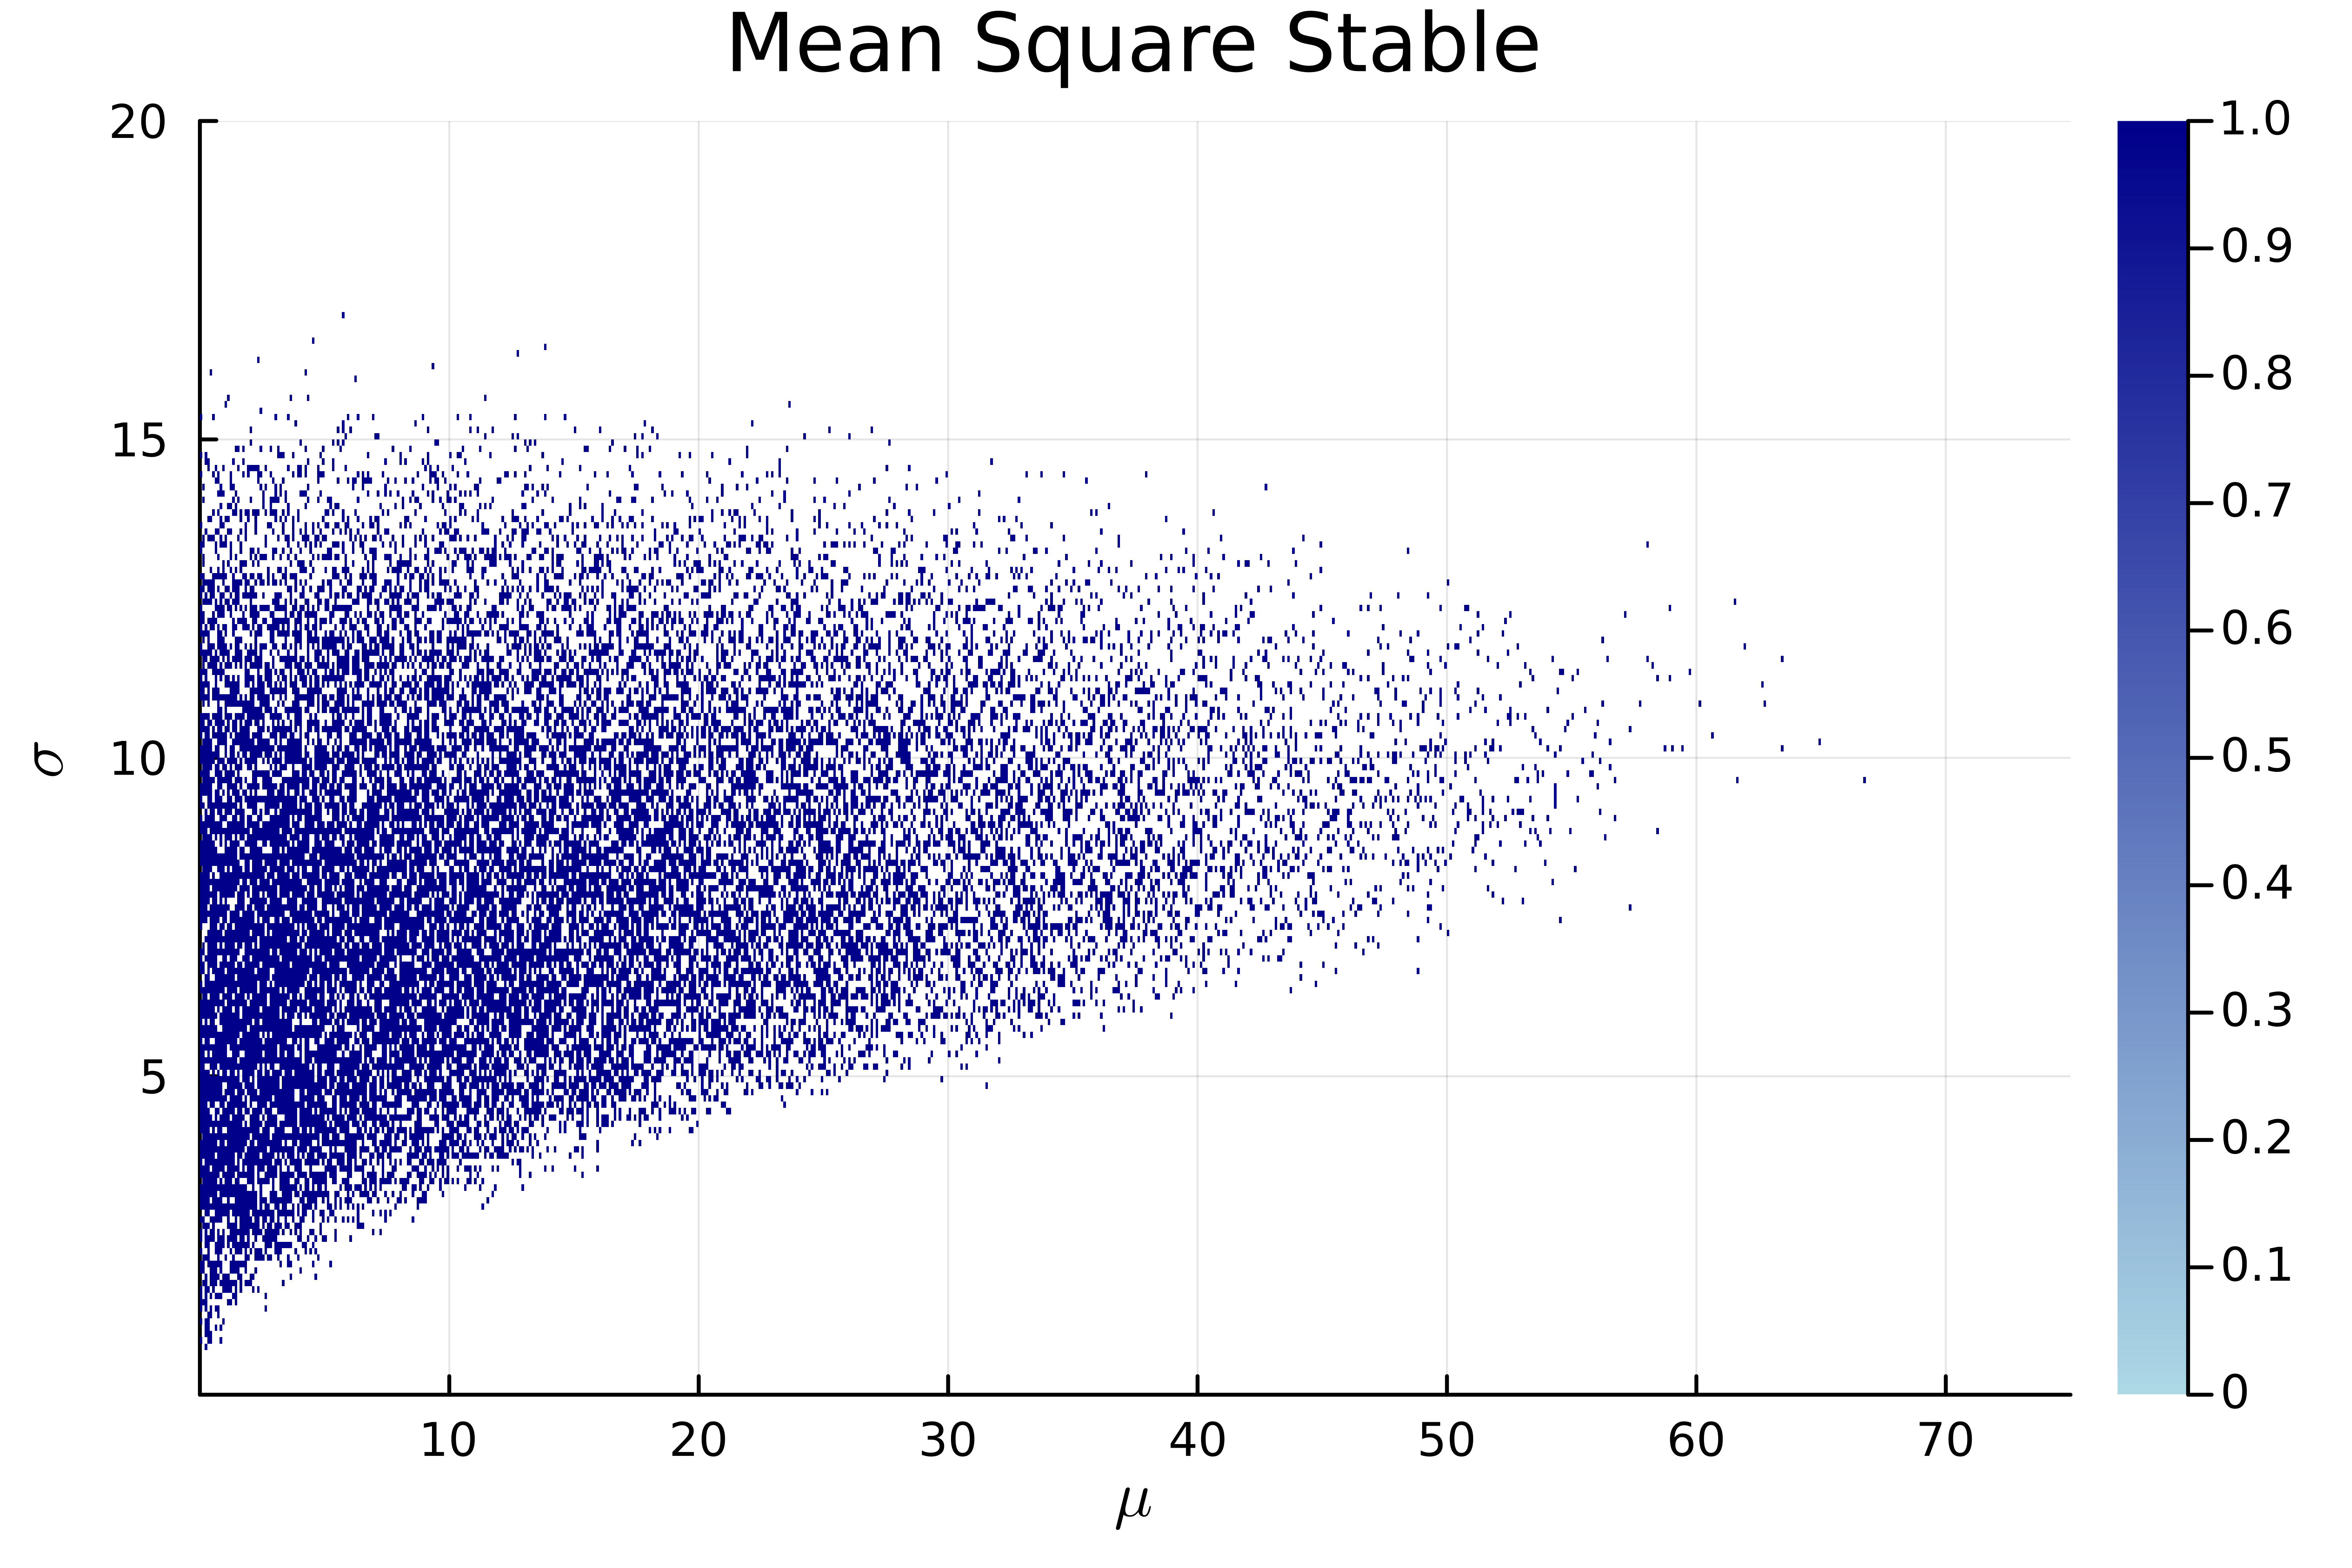
\includegraphics[scale=0.05]{imgs/4mean_square_stable.png}
    \caption{Mean Square Stable Values}
    \label{fig:meansq}
\end{figure}



\section*{Question 5}

An algorithm to simulate exit times for the SDE:


\begin{algorithmic}[1]
    \State Choose a step size $\Delta t$
    \State Choose some paths, $M$
    \For{$s = 1$ to $M$}
        \State Set $t_n = 0$ and $X_n = X_0$
        \While{$X_n > a$ and $X_n < b$}
            \State Compute a $N(0,1)$ sample $\xi_n$
            \State Replace $X_n$ by $X_n + \mu X_n \Delta t + \sigma X_n \xi_n$
            \State Replace $t_n$ by $t_n + \Delta t$
        \EndWhile
        \State Set $T_s^{exit} = t_n - 1/2 \Delta t$
    \EndFor
    \State Set $a_M = \frac{1}{M} \sum_{s=1}^{M} T_s^{exit}$
    \State Set $b^2_M = \frac{1}{M-1} \sum_{s=1}^{M} (T_s^{exit} - a_M)^2$
\end{algorithmic}

\begin{figure}[H]
            \centering
            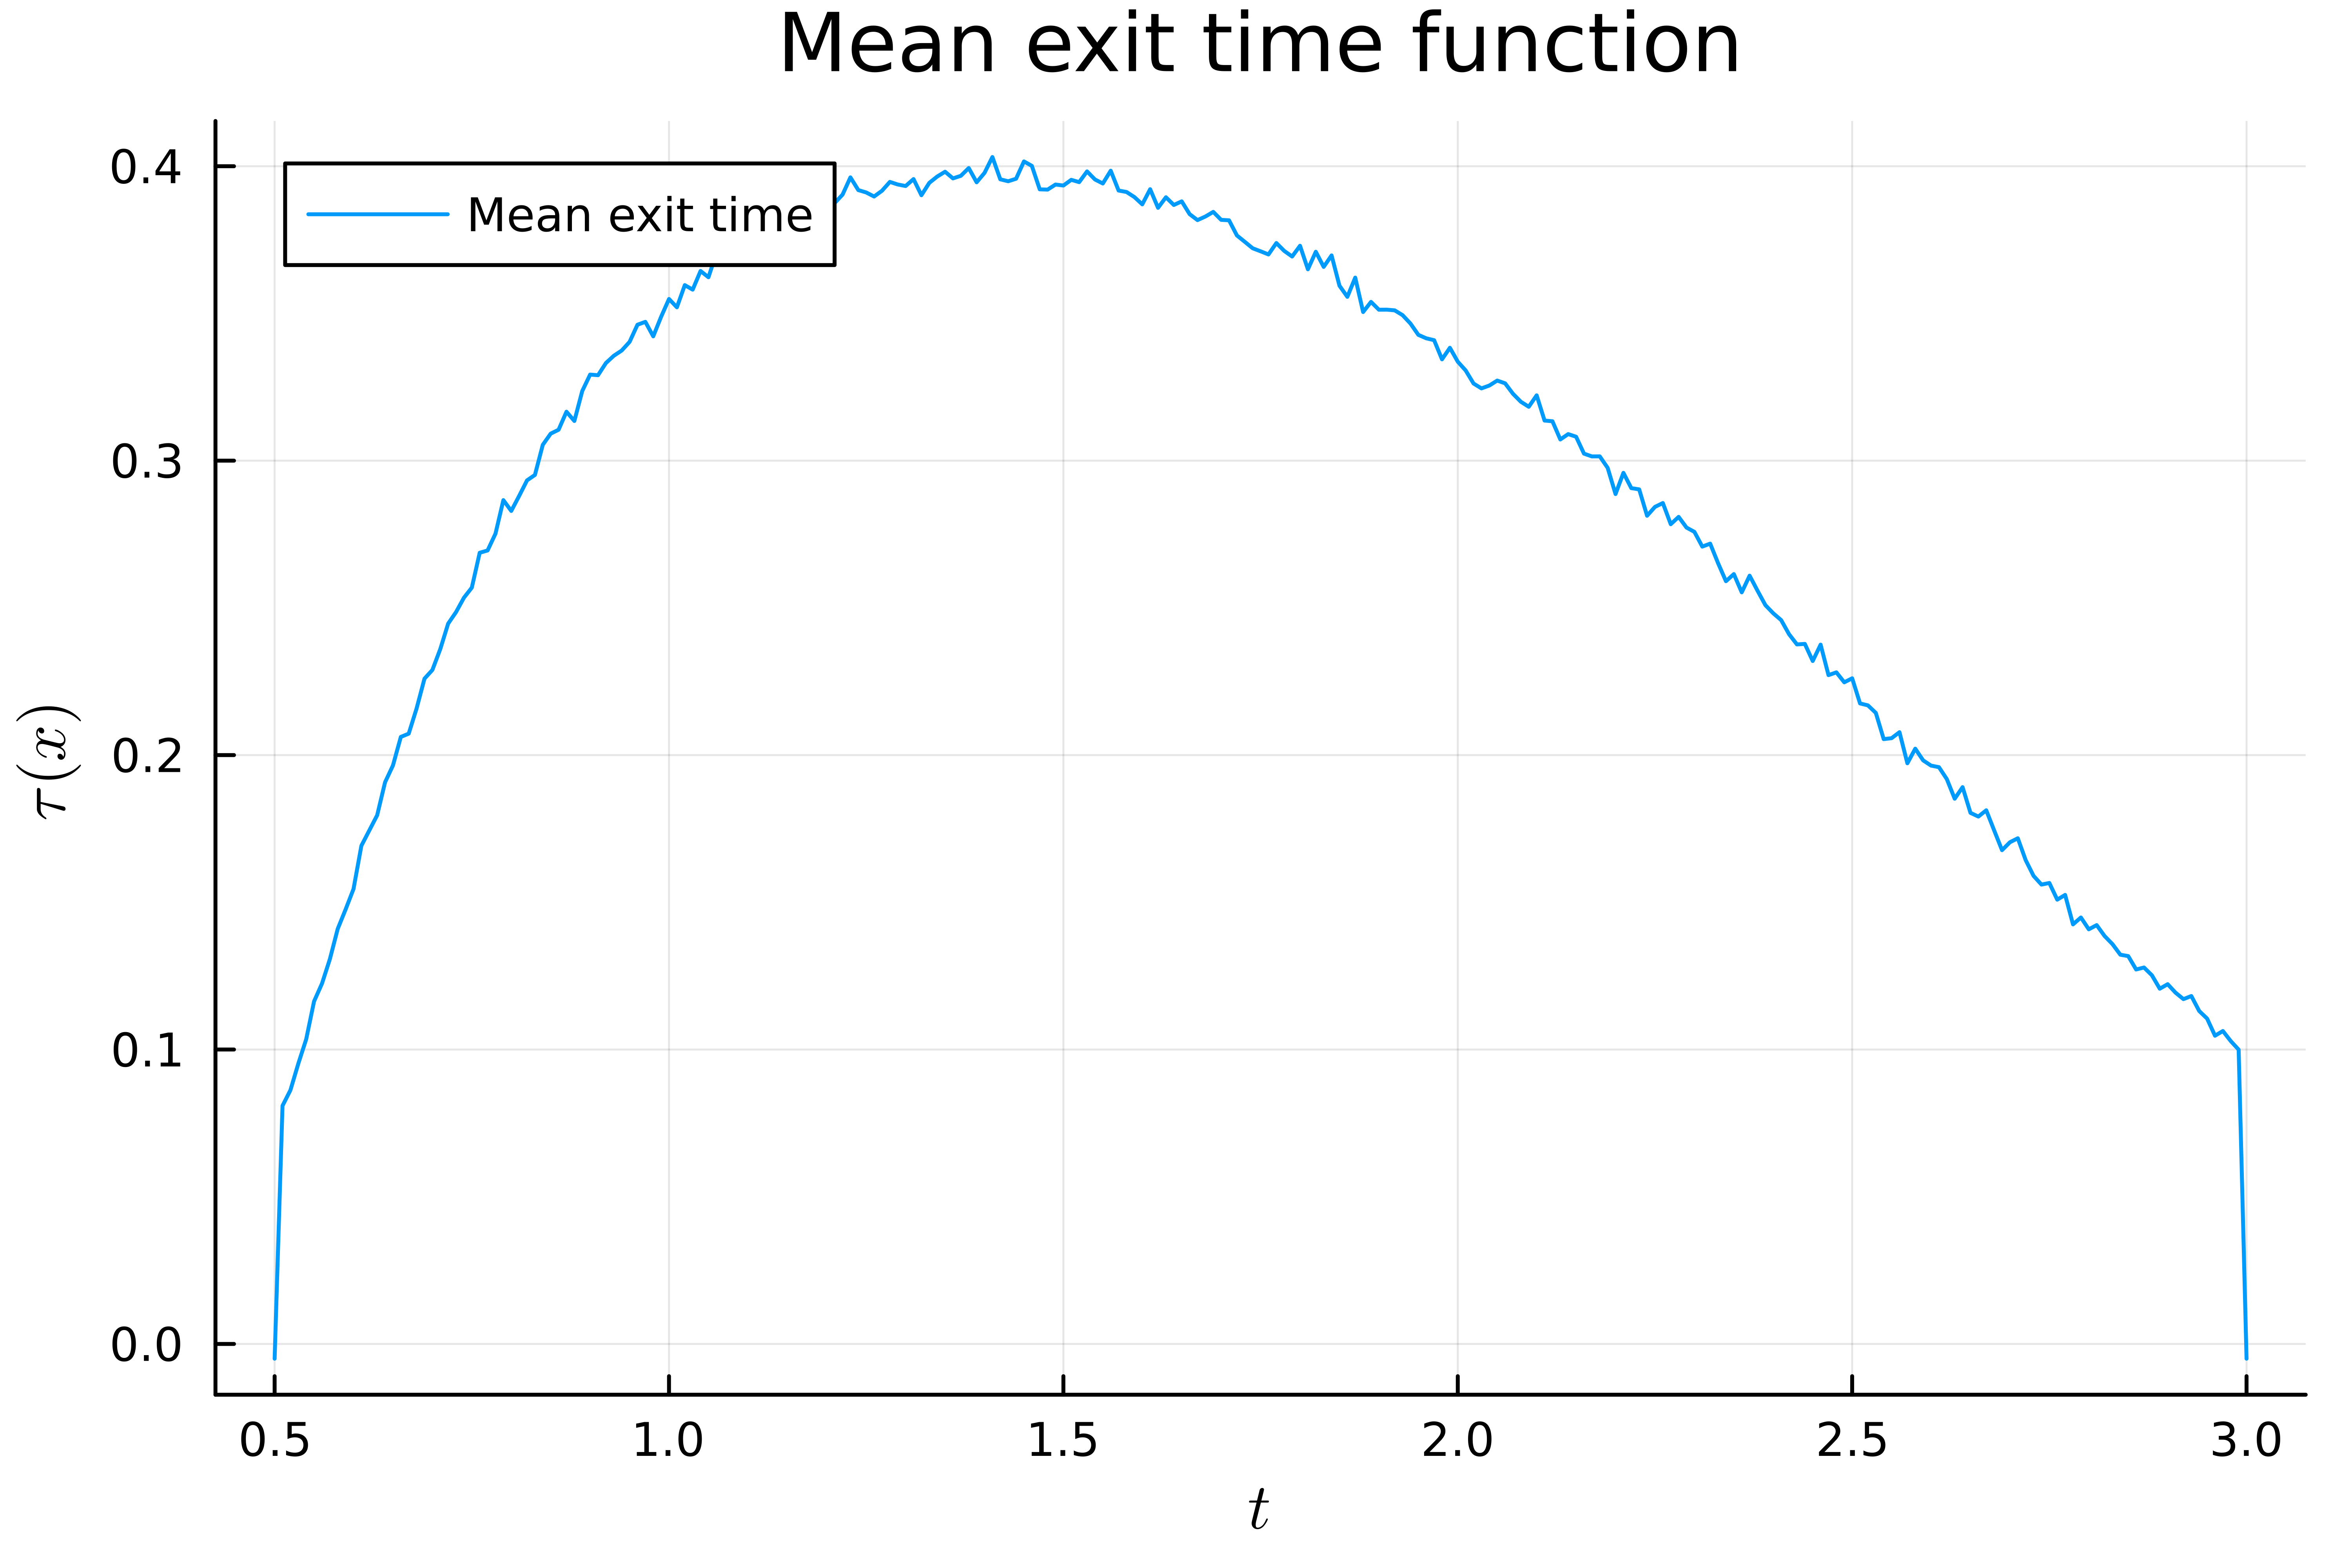
\includegraphics[scale=0.05]{imgs/5mean_exit_time.png}
            \caption{5}
            \label{fig:5}
      \end{figure}

      \begin{figure}[H]
            \centering
            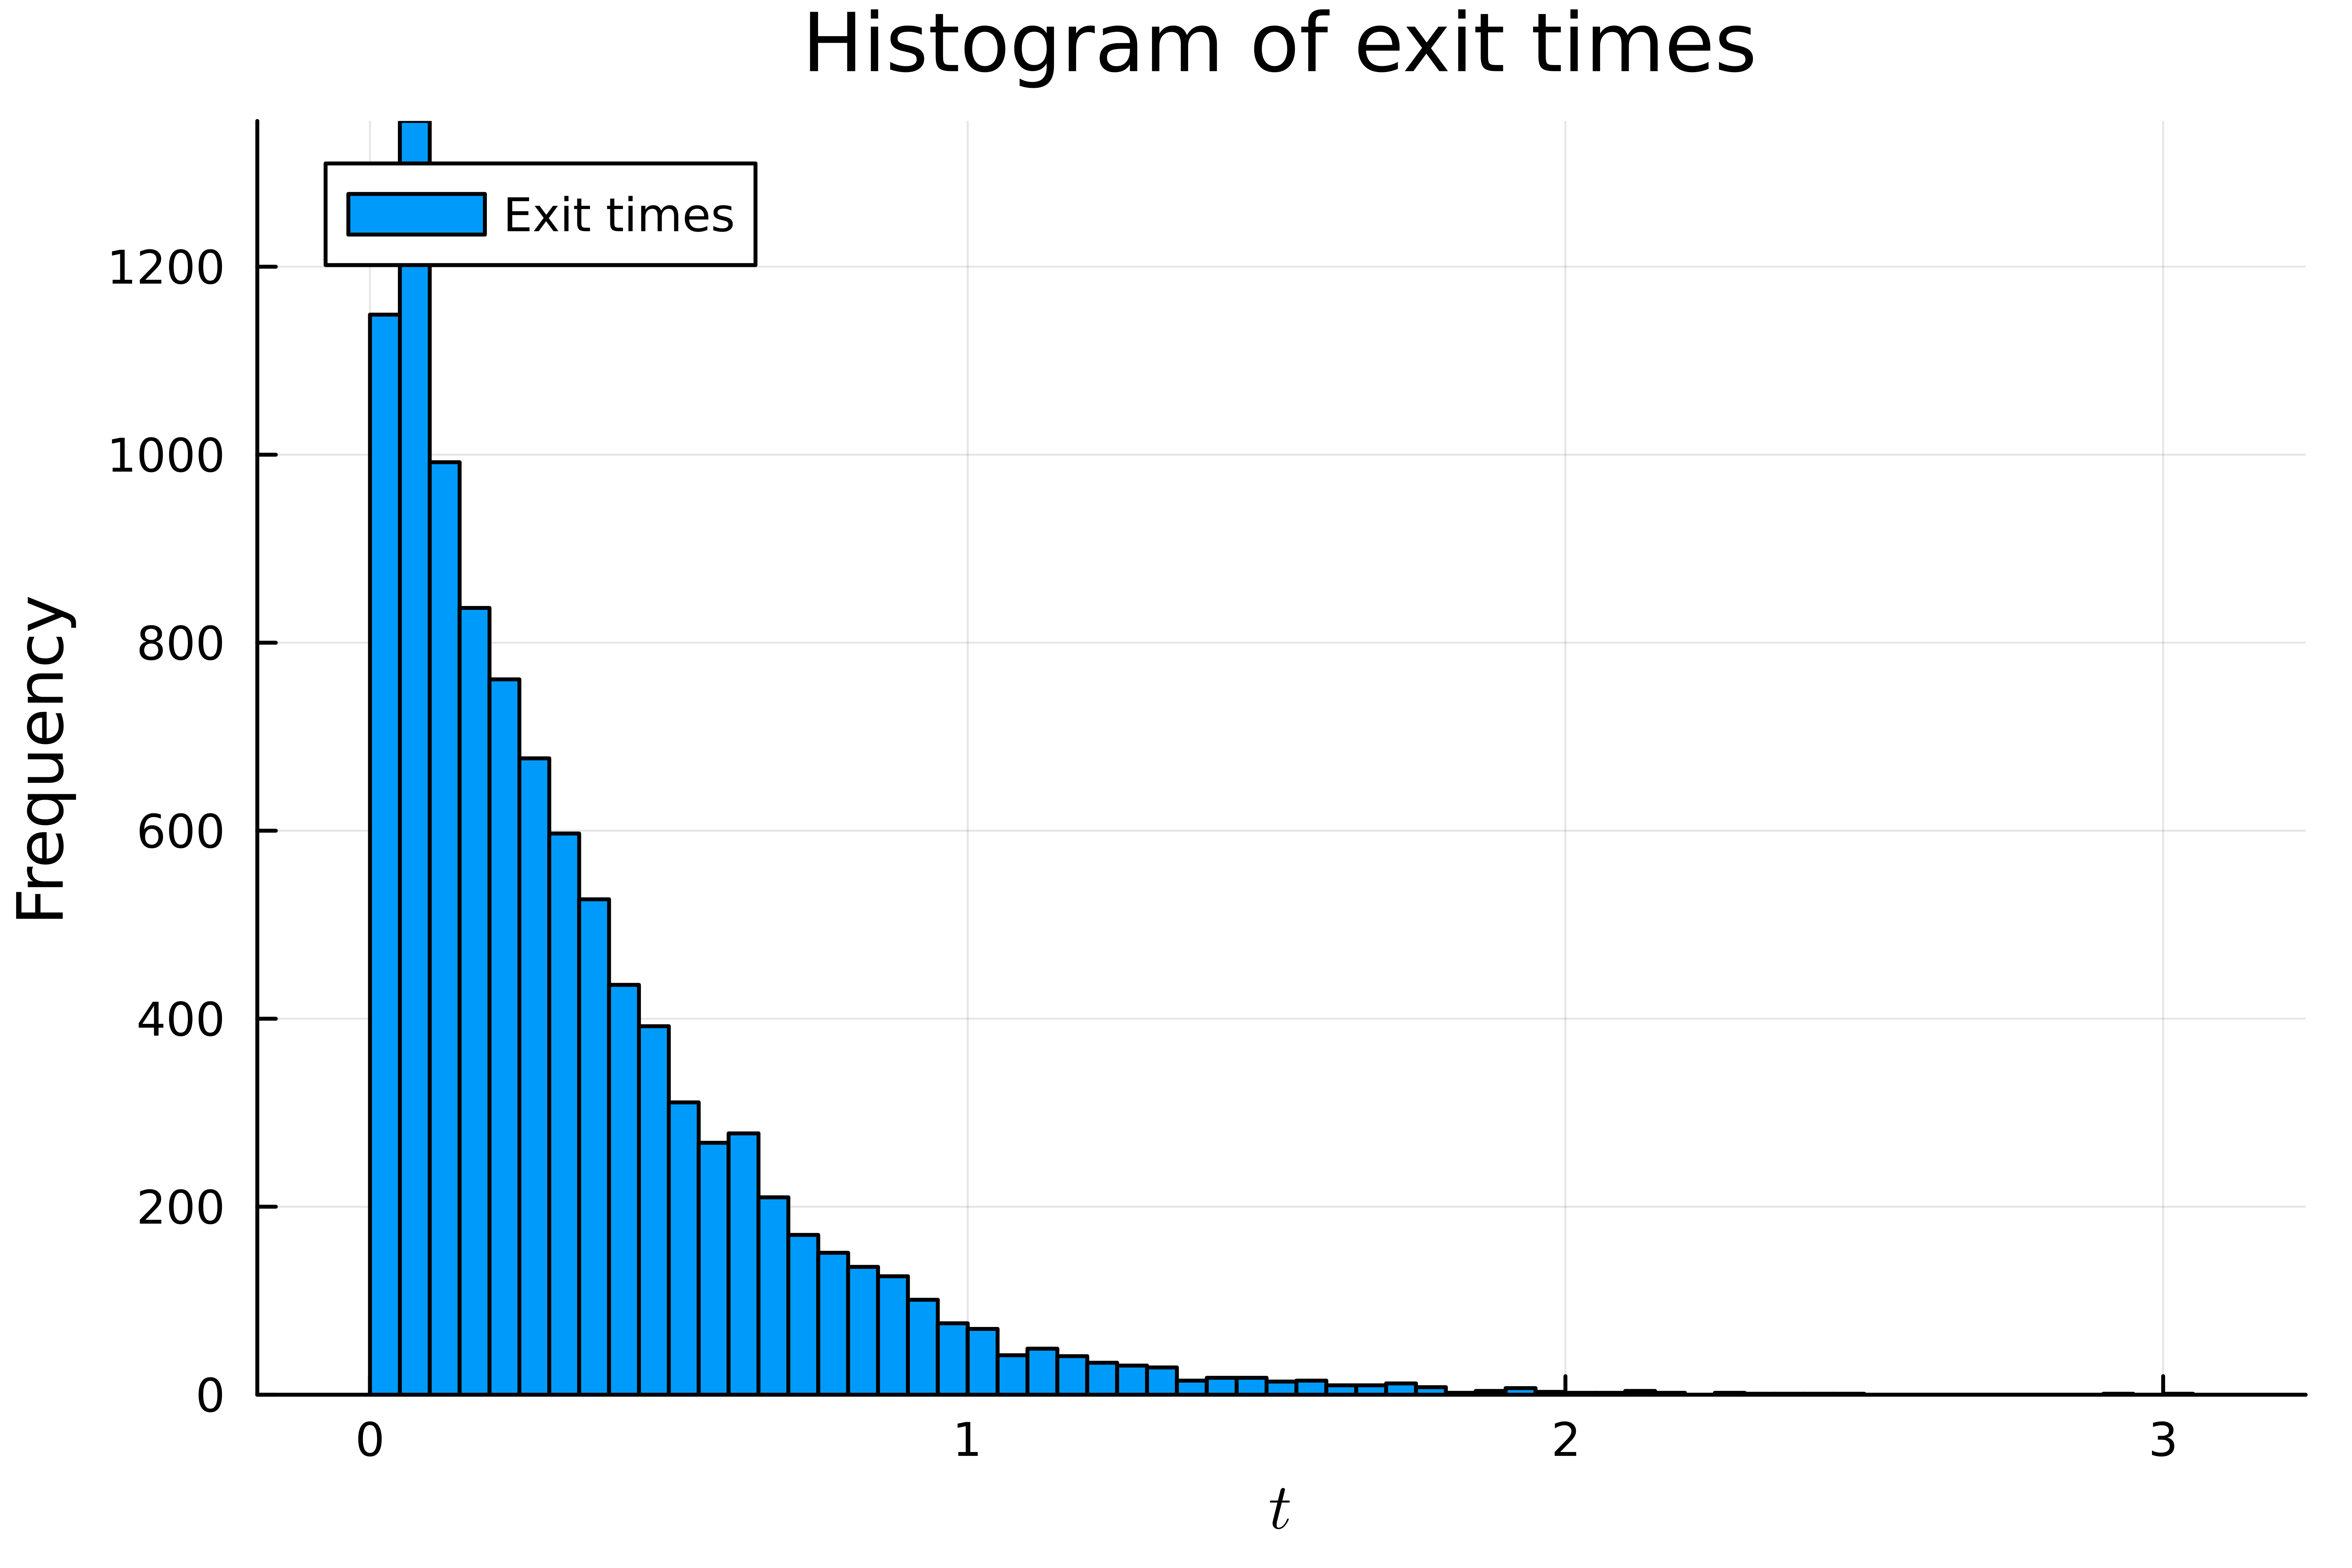
\includegraphics[scale=0.05]{imgs/5exit_times_histogram.png}
            \caption{5}
            \label{fig:5_exittimeshist}
      \end{figure}


\end{document}